% Adjust these for the path of the theme and its graphics, relative to this file
%\usepackage{beamerthemeFalmouthGamesAcademy}
\usepackage{../../beamerthemeFalmouthGamesAcademy}
\usepackage{multimedia}
\graphicspath{ {../../} }

% Default language for code listings
\lstset{language=Python
}

% For strikethrough effect
\usepackage[normalem]{ulem}
\usepackage{wasysym}

\usepackage{pdfpages}

% http://www.texample.net/tikz/examples/state-machine/
\usetikzlibrary{arrows,automata}

\newcommand{\modulecode}{COMP260}\newcommand{\moduletitle}{Distributed Systems}\newcommand{\sessionnumber}{5}

\begin{document}
\title{\sessionnumber: Exceptions and debugging}
\subtitle{\modulecode: \moduletitle}

\frame{\titlepage} 

\begin{frame}
	\frametitle{Learning outcomes}
	\begin{itemize}
		\item \textbf{Explain} the usefulness of exceptions and assertions in writing robust software
\item \textbf{Write} Python programs that throw and catch exceptions
\item \textbf{Use} the PyCharm debugger to trace the execution of programs
	\end{itemize}
\end{frame}

\begin{frame}{Reading}
	E.\ Dijkstra, 1968.
	Go To Statement Considered Harmful.
	\emph{Communications of the ACM},
	11(3):147--148.
\end{frame}

\part{Modular program design}
\frame{\partpage}

\begin{frame}[fragile]{Modular program design}
    \begin{itemize}
        \item We saw in session~9 that \textbf{splitting your code into several files} is generally a good idea \pause
        \item Python makes it easy: any .py file can be \lstinline[language=Python]{import}ed on demand \pause
        \item C++ is a little trickier...
    \end{itemize}
\end{frame}

\begin{frame}[fragile]{Definitions and declarations}
    A function \textbf{definition} specifies its name, return type, parameters, and the code it contains:
    \begin{lstlisting}
double average(double n1, double n2)
{
    return (n1 + n2) / 2.0;
}
    \end{lstlisting}
    \pause
    A function \textbf{declaration} specifies everything \textbf{except} the code:
    \begin{lstlisting}
double average(double n1, double n2);
    \end{lstlisting}
    \pause
    A declaration tells the compiler that this function exists, but is defined \textbf{elsewhere}
\end{frame}

\begin{frame}[fragile]{Sources and headers}
    \begin{itemize}
        \item A C++ project contains two main types of file \pause
        \item \textbf{Source files} (.cpp) usually contain \textbf{definitions} \pause
        \item \textbf{Header files} (.h) usually contain \textbf{declarations} \pause
        \item For example, \texttt{myfile.cpp} may contain some function definitions,
            and \texttt{myfile.h} may contain the declarations for those functions \pause
        \item (Yep, that means you have to type the same thing twice in two different files...)
    \end{itemize}
\end{frame}

\begin{frame}[fragile]{Example from last week}
    words.cpp
    \begin{lstlisting}
void readWords()
{
    std::cout << "Reading word list" << std::endl;
    // code omitted
}

std::string chooseRandomWord()
{
    // code omitted
}
    \end{lstlisting}
    
    words.h
    \begin{lstlisting}
#pragma once

void readWords();
std::string chooseRandomWord();
    \end{lstlisting}
\end{frame}

\begin{frame}[fragile]{Example from last week}
    \begin{itemize}
        \item \lstinline{readWords()} and \lstinline{chooseRandomWord()} are \textbf{defined} in \texttt{words.cpp} \pause
        \item \lstinline{readWords()} and \lstinline{chooseRandomWord()} are \textbf{declared} in \texttt{words.h} \pause
        \item Any file which does \lstinline{#include "words.h"} can call these functions as if they were declared in that file
    \end{itemize}
\end{frame}

\begin{frame}[fragile]{How \#include works}
    \begin{itemize}
        \item \lstinline{#include} works \textbf{exactly} as if the \lstinline{#include}d file were copied and pasted
            at the point where the \lstinline{#include} directive appears \pause
        \item All header files should start with \lstinline{#pragma once} --- otherwise,
            \lstinline{#include}ing the same file more than once will result in duplicate declaration errors \pause
        \item Putting an \lstinline{#include} directive in the wrong place (e.g.\ inside a function) will result in
            weird compile errors
    \end{itemize}
\end{frame}

\part{Exceptions}
\frame{\partpage}

\begin{frame}{Exceptions}
	\begin{itemize}
		\pause\item You've all seen them already...
	\end{itemize}
	\begin{center}
		\pause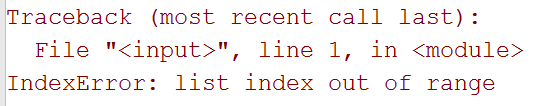
\includegraphics[width=0.5\textwidth]{exception}
	\end{center}
	\begin{itemize}
		\pause\item Some operations in a program can fail
		\pause\item Exceptions are a way of signalling that failure
	\end{itemize}
\end{frame}

\begin{frame}[fragile]{Raising exceptions}
	\pause
	\begin{lstlisting}
def factorial(n):
    if n < 0:
        raise ValueError("Argument must be positive")
	\end{lstlisting}
	\begin{itemize}
		\pause\item \lstinline{ValueError} is a built-in class
		\pause\item Its initialiser takes one argument: a human-readable
			string describing the error
		\pause\item The exception is an \textbf{instance} of the
			\lstinline{ValueError} class
	\end{itemize}
\end{frame}

\begin{frame}{Built-in exception types}
	\footnotesize\url{https://docs.python.org/2/library/exceptions.html}
\end{frame}

\begin{frame}[fragile]{Custom exception types}
	\pause
	\begin{lstlisting}
class UnreticulatedSplineError(Exception):
    def __init__(self, message):
		    Exception.__init__(self, message)

...
if not spline.is_reticulated():
    raise UnreticulatedSplineError("Spline must be reticulated")
	\end{lstlisting}
	\begin{itemize}
		\pause\item Inherit from built-in class \lstinline{Exception}
		\pause\item Just like any other class --- can contain any required
			fields and methods
	\end{itemize}
\end{frame}

\begin{frame}[fragile]{Catching exceptions}
	\begin{lstlisting}
try:
    input_file = open(filename, "rt")
except IOError:
    print "Failed to open file, please select a different one"
	\end{lstlisting}
	\begin{itemize}
		\pause\item If anything inside the \lstinline{try} block throws an
			\lstinline{IOError} (or a subclass of \lstinline{IOError}),
			the \lstinline{except} block executes
		\pause\item A \lstinline{try} block can have several \lstinline{except}
			blocks for different exception types
		\pause\item An uncaught exception kills the program
	\end{itemize}
\end{frame}

\begin{frame}{Exceptions and control flow}
	\begin{itemize}
		\pause\item Raising exception transfers control to the innermost matching
			\lstinline{except} handler
		\pause\item This can result in breaking out of loops and functions
		\pause\item This can be powerful in the hands of a good programmer...
		\pause\item ... or confusing in the hands of a bad one
	\end{itemize}
\end{frame}

\begin{frame}{Types of exceptions}
	There are two types of exceptions...
	\begin{itemize}
		\pause\item Those intended to catch \textbf{runtime errors}
			(e.g.\ missing files, insufficient resources, invalid input, ...)
			\begin{itemize}
				\pause\item Good software should \textbf{catch} and \textbf{recover} from these
			\end{itemize}
		\pause\item Those intended to catch \textbf{programmer errors}
			(e.g.\ type mismatch, index out of bounds, divide by zero, ...)
			\begin{itemize}
				\pause\item Generally best to let these crash the program so that the programmer can notice and fix them
				\pause\item A commercially released program might catch them to allow the user to submit a bug report to the developer
			\end{itemize}
	\end{itemize}
\end{frame}

\begin{frame}[fragile]{Assertions}
	\begin{itemize}
		\pause\item \lstinline{AssertionError} is a special exception type for catching programmer errors
		\pause\item Can be raised with the following syntax:
	\end{itemize}
	\begin{lstlisting}
assert n > 0, "n must be positive"
	\end{lstlisting}
	\begin{itemize}
		\pause\item The exception is raised if the condition is \lstinline{False}
		\pause\item \lstinline{assert} should \textbf{only} be used to catch programmer errors,
			therefore you should \textbf{never} try to handle \lstinline{AssertionError} in a \lstinline{try ... except}
			block
		\pause\item In some programming languages, assertions are stripped out of ``Release'' builds ---
			so avoid assertions with side-effects!
	\end{itemize}
\end{frame}

\begin{frame}[fragile]{More options with try blocks}
	\begin{lstlisting}
try:
    input_file = open(filename, "rt")
except IOError as err:
    print "File error:", err
else:
    print "This only executes if the try block did not raise an exception"
finally:
    print "This executes whether or not the try block raised an exception, even if there were uncaught exceptions"
	\end{lstlisting}
\end{frame}

\begin{frame}[fragile]{It's easier to ask forgiveness than permission}
	\pause I.e.\ it's better to catch exceptions
		than to use \lstinline{if} statements to avoid them
	\pause\begin{lstlisting}
try:
    x = list[index]
except IndexError:
    x = None
	\end{lstlisting}
	This is ``more Pythonic'' than this:
	\pause\begin{lstlisting}
if index >= 0 and index < len(list):
    x = list[index]
else:
    x = None
	\end{lstlisting}
\end{frame}

\part{Debugging}
\frame{\partpage}

\begin{frame}{OpenGL Error States}
	\begin{itemize}
		\pause\item \lstinline{glGetError()} queries behind-the-scenes error flags to check state.
		\pause\item Possible \lstinline{glEnum} error codes for each function are listed in the documentation, e.g. for glBindTexture:
	\end{itemize}
	\begin{figure}[h!]
		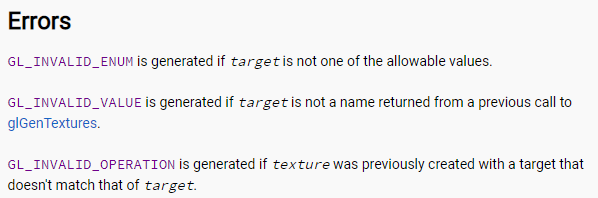
\includegraphics[width=0.8\textwidth]{glerrors}
	\end{figure}
\end{frame}

\begin{frame}[fragile]{Debug Output}
	\begin{itemize}
		\pause\item Extension made core feature from v4.3
		\pause\item Includes information about the cause and severity.
	\end{itemize}
	\pause\begin{lstlisting}
SDL_GL_SetAttribute(SDL_GL_CONTEXT_FLAGS,
		SDL_GL_CONTEXT_DEBUG_FLAG);	// Set up debug context
glEnable(GL_DEBUG_OUTPUT);
glEnable(GL_DEBUG_OUTPUT_SYNCHRONOUS);
glDebugMessageCallback(debugMessage, NULL);
glDebugMessageControl(GL_DONT_CARE, GL_DONT_CARE,
		GL_DONT_CARE, 0, NULL, GL_TRUE);	// Filter errors

// Callback
void APIENTRY debugMessage(GLenum source, GLenum type,
	GLuint id, GLenum severity, GLsizei length,
	const GLchar *message, const void *userParam) {
	// Do something with the error info
	// (print, write to file etc.)
}
	\end{lstlisting}
\end{frame}

\begin{frame}{Debugging Shaders}
	\begin{itemize}
		\pause\item Basic information from \textbf{compilation error reports}.
		\pause\item OpenGL GLSL \textbf{reference compiler} tests shader code against OpenGL specification.
		\pause\item Can use \textbf{colour channels} to display values.
		\pause\item Display \textbf{framebuffer contents} in the corner of the screen (similar to post-processing setup).
		\pause\item More detailed inspection requires using a \textbf{3rd party tool} (depending on GPU vendor etc.).
	\end{itemize}
\end{frame}

\part{Worksheet D}
\frame{\partpage}

\end{document}
